%%%%%%%%%%%%%%%%%%%%%%%%%%%%%%%%%%%%%%%%%
% Thin Sectioned Essay
% LaTeX Template
% Version 1.0 (3/8/13)
%
% This template has been downloaded from:
% http://www.LaTeXTemplates.com
%
% Original Author:
% Nicolas Diaz (nsdiaz@uc.cl) with extensive modifications by:
% Vel (vel@latextemplates.com)
%
% License:
% CC BY-NC-SA 3.0 (http://creativecommons.org/licenses/by-nc-sa/3.0/)
%
%%%%%%%%%%%%%%%%%%%%%%%%%%%%%%%%%%%%%%%%%

%----------------------------------------------------------------------------------------
%	PACKAGES AND OTHER DOCUMENT CONFIGURATIONS
%----------------------------------------------------------------------------------------

\documentclass[letterpaper,10pt]{article} % Font size (can be 10pt, 11pt or 12pt) and paper size (remove a4paper for US letter paper)
\usepackage{geometry}
\geometry{paperwidth=4in,margin=.1in,paperheight=65in}
\usepackage[protrusion=true,expansion=true]{microtype} % Better typography
\usepackage{graphicx} % Required for including pictures
\usepackage{caption}
\usepackage{subcaption}
\usepackage{wrapfig} % Allows in-line images
\usepackage{amsmath,amsthm}
\usepackage{thmtools}
\usepackage{mathpazo} % Use the Palatino font
\usepackage[T1]{fontenc} % Required for accented characters
\linespread{1.05} % Change line spacing here, Palatino benefits from a slight increase by default

\makeatletter
\newcommand{\pipe}{\;\middle\vert\;}
\newcommand{\condp}[2]{\Pr\left( #1 \pipe #2 \right)}
\newcommand{\pr}[1]{\Pr\left( #1 \right)}
\newcommand{\condpe}[2]{\frac{\pr{#1,#2}}{\pr{#2}}}
\newcommand{\condpb}[2]{\frac{\condp{#2}{#1}\pr{#1}}{\pr{#2}}}
\newcommand{\norm}[1]{\left|#1\right|}
\DeclareMathOperator*{\argmin}{arg\,min}
\DeclareMathOperator*{\argmax}{arg\,max}
%theorem styling
\declaretheorem{theorem} 
\declaretheoremstyle[%
spaceabove=-6pt,%
spacebelow=6pt,%
headfont=\normalfont\itshape,%
postheadspace=1em,%
qed=\qedsymbol,%
headpunct={}
]{mystyle} 
\declaretheorem[name={},style=mystyle,unnumbered,
]{Proof}

\newcommand{\prove}[1]{
\begin{Proof}
\begin{align*}
#1
\end{align*}
\end{Proof}
}

\renewcommand{\@listI}{\itemsep=0pt} % Reduce the space between items in the itemize and enumerate environments and the bibliography

\renewcommand{\maketitle}{ % Customize the title - do not edit title and author name here, see the TITLE block below
\begin{flushright} % Right align
{\LARGE\@title} % Increase the font size of the title

{\large\@author} % Author name
\\\@date % Date

\end{flushright}
}

%----------------------------------------------------------------------------------------
%	TITLE
%----------------------------------------------------------------------------------------

\title{\textbf{Assignment 1}\\ % Title
Machine Learning 10-701} % Subtitle

\author{\textsc{Arjun Menon} % Author
\\{\textit{Carnegie Mellon University}}} % Institution

%----------------------------------------------------------------------------------------

\begin{document}

\maketitle % Print the title section

\section{Classification [Dougal]}
\subsection{Drawing decision boundaries}

\begin{figure}[h]
\centering
\begin{subfigure}[b]{\textwidth}
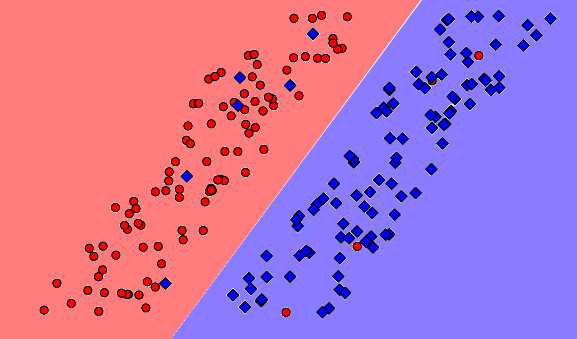
\includegraphics[width=\textwidth]{handout/q3-1-logistic}
\caption{Logistic Regressor decision boundary}
\label{fig:log1}
\end{subfigure}%

\begin{subfigure}[b]{\textwidth}
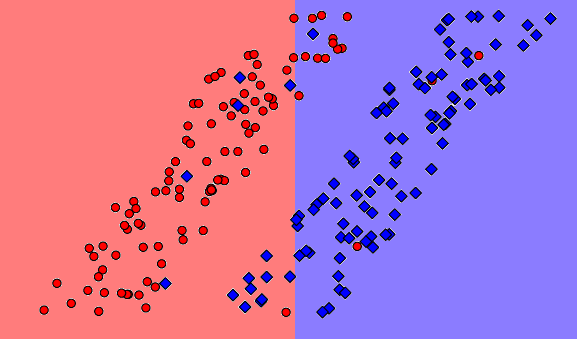
\includegraphics[width=\textwidth]{handout/q3-1-bayes}
\caption{Naive Bayes decision boundary}
\label{fig:bayes1}
\end{subfigure}

\begin{subfigure}[b]{\textwidth}
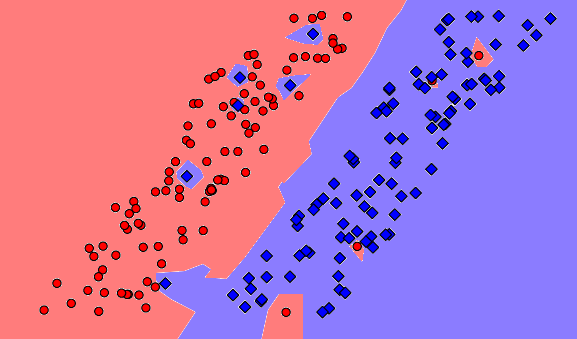
\includegraphics[width=\textwidth]{handout/q3-1-NN}
\caption{1-NN decision boundary}
\label{fig:1nn1}
\end{subfigure}

\begin{subfigure}[b]{\textwidth}
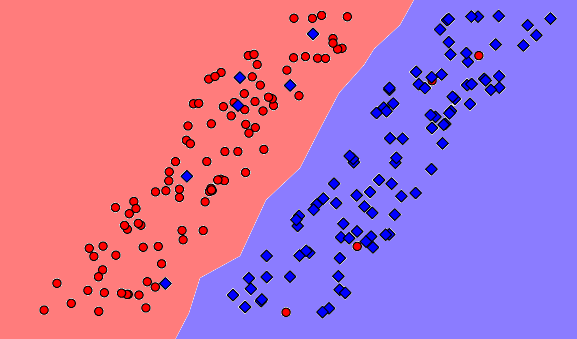
\includegraphics[width=\textwidth]{handout/q3-1-10NN}
\caption{10-NN decision boundary}
\label{fig:10nn1}
\end{subfigure}

\caption{Decision boundaries of the first data set}\label{fig:decision1}
\end{figure}

In Figure~\ref{fig:decision1} we can see the decision boundaries on the first data set. 

Figure~\ref{fig:log1} shows the logistic regression boundary which liear between the two sets. 

Figure~\ref{fig:bayes1} shows that Naive Bayes performs poorly on this data set because the features are NOT independant of each other. One feature becomes completely irrelevant to classification.

Figure~\ref{fig:1nn1} shows that 1-NN is very sensitive to the noise, and creates strange voronoi regions where it provides the obviously wrong label.

Figure~\ref{fig:10nn1} shows 10-NN performing very well on noise, and providing a boundary similar to the logistic regressor.

\begin{figure}[h]
\centering
\begin{subfigure}[b]{\textwidth}
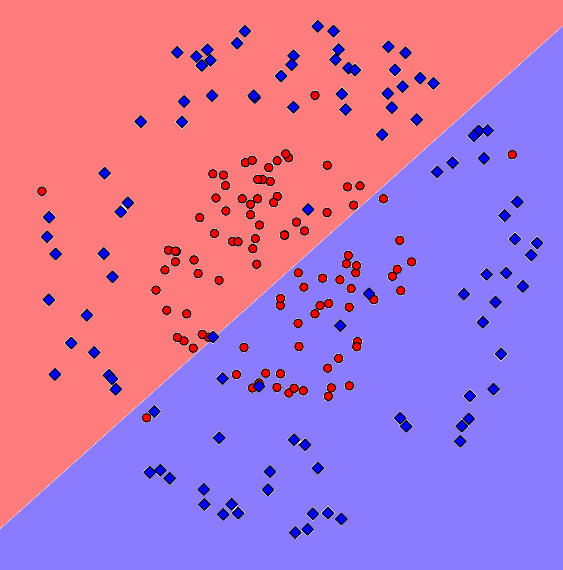
\includegraphics[width=\textwidth]{handout/q3-2-logistic}
\caption{Logistic Regressor decision boundary}
\label{fig:log2}
\end{subfigure}%

\begin{subfigure}[b]{\textwidth}
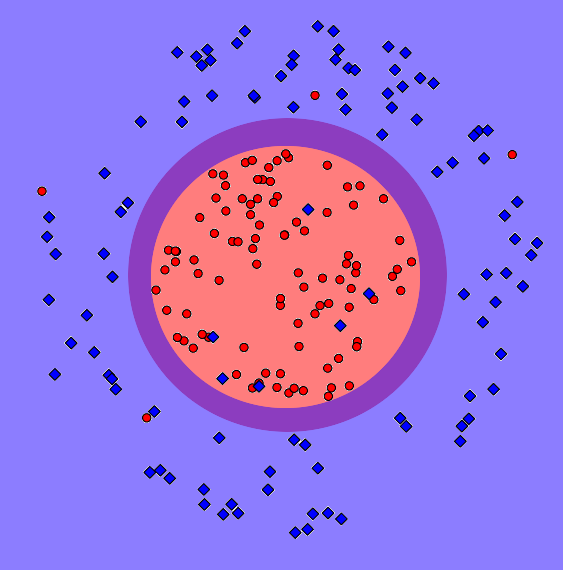
\includegraphics[width=\textwidth]{handout/q3-2-bayes}
\caption{Naive Bayes decision boundary}
\label{fig:bayes2}
\end{subfigure}

\begin{subfigure}[b]{\textwidth}
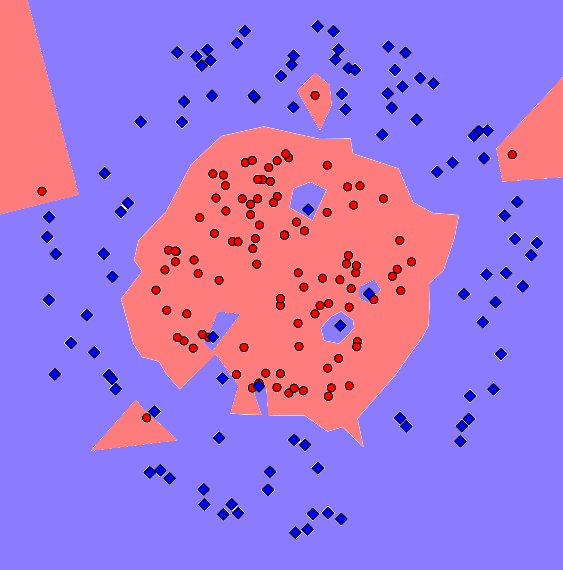
\includegraphics[width=\textwidth]{handout/q3-2-NN}
\caption{1-NN decision boundary}
\label{fig:1nn2}
\end{subfigure}

\begin{subfigure}[b]{\textwidth}
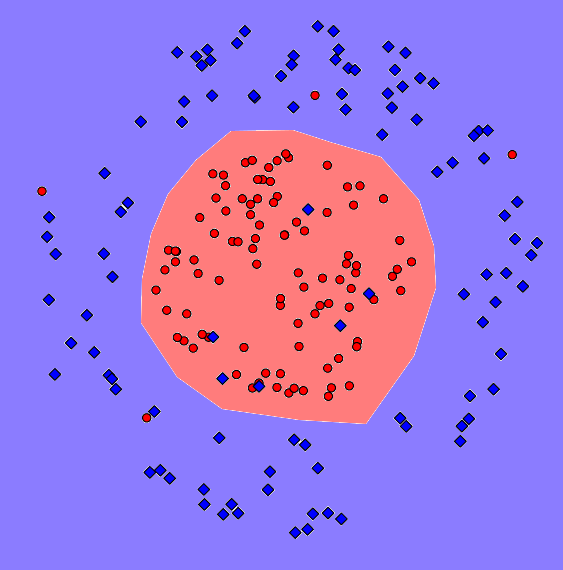
\includegraphics[width=\textwidth]{handout/q3-2-10NN}
\caption{10-NN decision boundary}
\label{fig:10nn2}
\end{subfigure}

\caption{Decision boundaries of the second data set}\label{fig:decision2}
\end{figure}

Figure~\ref{fig:decision2} shows the classifier decision boundaries on the circular data set.

Figure~\ref{fig:log2} shows the logistic regression decision boundary. Note that it is unable to find a line to seperate the data. It performs poorly on this data set.

Figure~\ref{fig:bayes2} shows the Naive Bayes classifier decision boundary creating roughly circular decision boundary. This is because the guassian for the red-data on both features are highly kurtotic so for when posterior probability for red is high are represented by a roughly circular region. The purple region is where the decision boundary is roughly located. It can take any shape within that region.

Figure~\ref{fig:1nn2} shows the 1-NN classifier decision boundary. You can see that the same sensitivity to noise occurs, and huge voronoi regision of red appear on the peripherry.

Figure~\ref{fig:10nn2} shows the 10-NN classifier decision boundary which is robust to noise and has no patches like in 1-NN.

\subsection{Defeating classifiers}

\begin{figure}[h]
\centering
\begin{subfigure}[b]{\textwidth}
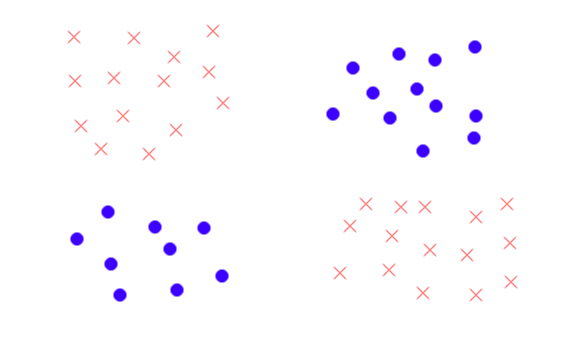
\includegraphics[width=\textwidth]{handout/3-2/logistic1}
\caption{Logistic Regressor failure case 1}
\label{fig:faillr1}
\end{subfigure}%

\begin{subfigure}[b]{\textwidth}
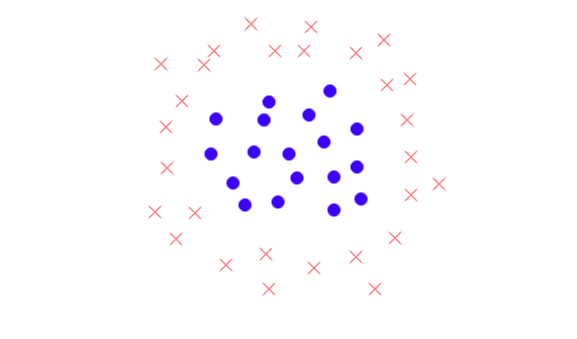
\includegraphics[width=\textwidth]{handout/3-2/logistic2}
\caption{Logistic Regressor failure case 2}
\label{fig:faillr2}
\end{subfigure}

\begin{subfigure}[b]{\textwidth}
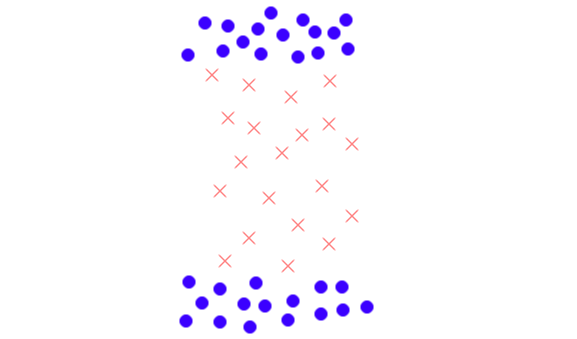
\includegraphics[width=\textwidth]{handout/3-2/logistic3}
\caption{Logistic Regressor failure case 3}
\label{fig:faillr3}
\end{subfigure}

\caption{Failure case datasets for }\label{fig:faillr}
\end{figure}

Figure~\ref{fig:faillr} shows the failure case datasets for Logistic regression, which are described as follows:

\begin{itemize}
\item Figure~\ref{fig:faillr1} shows the "XOR" dataset. No linear seperator exists here for this problem, but the clusters are obvious to a human.
\item Figure~\ref{fig:faillr2} shows the data set in the previous sub question. It is unable to find a linear seperator here.
\item Figure~\ref{fig:faillr3} shows a made-up dataset, where the positive examples are put into two clusters, making it impossible for a line to separate it with, without crossing through the negative examples.
\end{itemize}

\begin{figure}[h!]
\centering
\begin{subfigure}[b]{\textwidth}
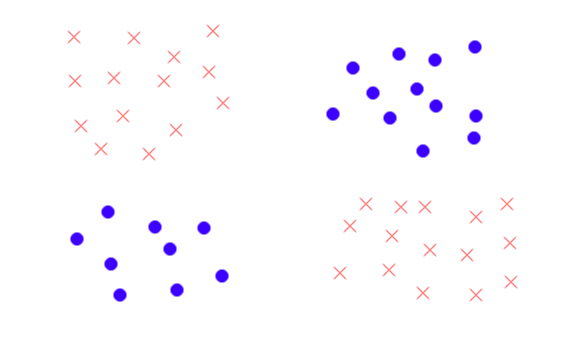
\includegraphics[width=\textwidth]{handout/3-2/bayes1}
\caption{Naive Bayes failure case 1}
\label{fig:failbayes1}
\end{subfigure}%

\begin{subfigure}[b]{\textwidth}
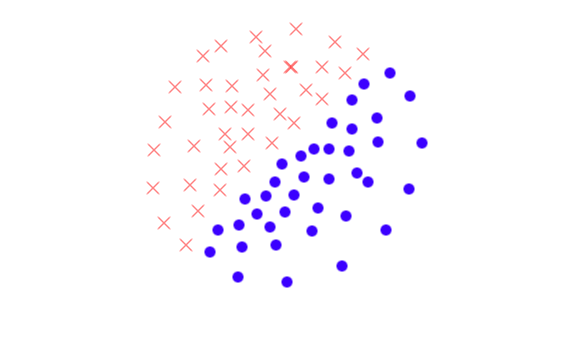
\includegraphics[width=\textwidth]{handout/3-2/bayes2}
\caption{Naive Bayes failure case 2}
\label{fig:failbayes2}
\end{subfigure}

\begin{subfigure}[b]{\textwidth}
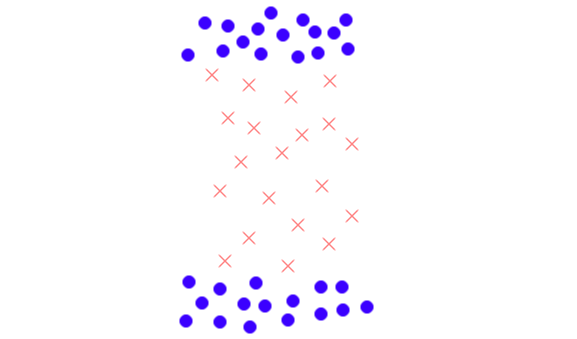
\includegraphics[width=\textwidth]{handout/3-2/bayes3}
\caption{Naive Bayes failure case 3}
\label{fig:failbayes3}
\end{subfigure}

\caption{Failure case datasets for }\label{fig:failbayes}
\end{figure}

Figure~\ref{fig:failbayes} shows the failure datasets for Naive Bayes where it cannot to much better than guessing at random. The datasets are described as follows.

\begin{itemize}
\item Figure~\ref{fig:failbayes1} gives the XOR dataset. Here the features are not captured by the gaussians. It would work if bimodal gaussians where used, but in this case the gaussians are blended together can don't give a good seperation.
\item Figure~\ref{fig:failbayes2} gives a half-circles dataset, where the equator is rotated by 45 degrees. The same instance of highly overlapping guassians occurs.
\item Figure~\ref{fig:failbayes3} gives the same made-up data set however it is possible to sample the data for the negative examples (red X's) such that an estimated guassian in the vertical feature has the same support as one constructed for the positive examples (blue O's).
\end{itemize}

\begin{figure}[h!]
\centering
\begin{subfigure}[b]{\textwidth}
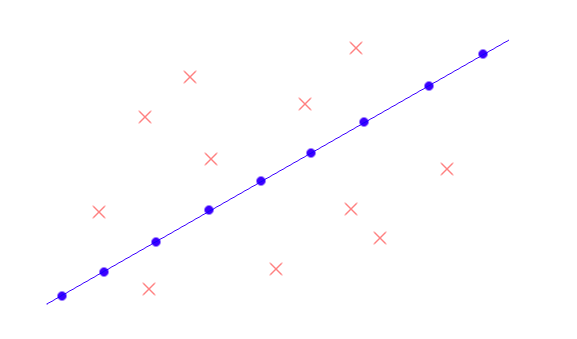
\includegraphics[width=\textwidth]{handout/3-2/NN1}
\caption{Nearest Neighbour failure case 1}
\label{fig:failnn1}
\end{subfigure}%

\begin{subfigure}[b]{\textwidth}
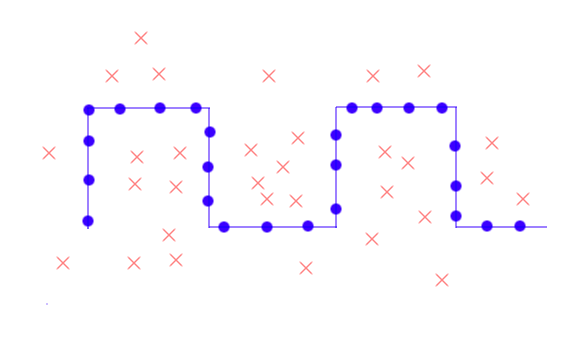
\includegraphics[width=\textwidth]{handout/3-2/NN2}
\caption{Nearest Neighbour failure case 2}
\label{fig:failnn2}
\end{subfigure}

\caption{Failure case datasets for }\label{fig:failnn}
\end{figure}

Figure~\ref{fig:failnn} shows the failure datasets for Nearest Neighbour where it cannot to much better than guessing at random. The datasets are described as follows:

\begin{itemize}
\item Figure~\ref{fig:failnn1} is the classification of points lie ON defined line. Here no matter how many positive examples (blue O's) you give for points on the line, it will classify that any given point lies off the line. This is unless the distance metric you choose somehow knows of distribution you're getting the data from.
\item Figure~\ref{fig:failnn2} is the classification of points on a square wave. This follows the same as the previous failure case.
\item The classification of Prime Numbers is not possible with NN as well. Positive examples are Primes, and negative examples are Non-primes.
\end{itemize}

%\bibliographystyle{unsrt}
%\bibliography{sample}

%----------------------------------------------------------------------------------------

\end{document}
